\documentclass[border=12pt,tikz]{standalone}
\usepackage[T1]{fontenc}
\usepackage{tikz}
\usetikzlibrary{positioning, arrows.meta, calc, fit, backgrounds, decorations.pathreplacing, shapes.geometric}

\definecolor{inputcol}{rgb}{0.17, 0.48, 0.71}
\definecolor{hiddencol}{rgb}{1.00, 0.50, 0.06}
\definecolor{outputcol}{rgb}{0.84, 0.15, 0.16}
\definecolor{frozencol}{rgb}{0.17, 0.63, 0.17}
\definecolor{ensemblecol}{rgb}{0.00, 0.75, 1.00}
\definecolor{residualcol}{rgb}{0.74, 0.74, 0.13}
\definecolor{directcol}{rgb}{0.55, 0.22, 0.08}
\definecolor{learnedcol}{rgb}{0.12, 0.30, 0.60}

\tikzset{
  ionode/.style={circle, draw, minimum size=6.5mm, inner sep=0pt,
                 font=\scriptsize, line width=0.45pt},
  input node/.style={ionode, fill=inputcol!20, draw=inputcol!70},
  output node/.style={ionode, fill=outputcol!20, draw=outputcol!70},
  tensor/.style={rectangle, draw, rounded corners=2pt,
                 minimum width=12mm, minimum height=25mm,
                 inner sep=3pt, font=\scriptsize, align=center,
                 line width=0.6pt},
  hidden block/.style={tensor, fill=hiddencol!15, draw=hiddencol!70},
  frozen block/.style={tensor, fill=frozencol!12, draw=frozencol!60},
  sum node/.style={circle, draw, minimum size=7mm, inner sep=0pt,
                   font=\normalsize, line width=0.5pt},
  avg node/.style={circle, draw, minimum size=7mm, inner sep=0pt,
                   font=\scriptsize, line width=0.5pt,
                   fill=ensemblecol!12},
  dots node/.style={font=\Large, inner sep=0pt},
  annot/.style={font=\scriptsize, text=black!65},
  lbl/.style={font=\scriptsize\bfseries,
              text=black!80, align=center},
  arr/.style={-{Stealth[length=2.5pt]}, line width=0.55pt, black!50},
  random arr/.style={arr, densely dashed, frozencol!70},
  learned arr/.style={arr, line width=0.9pt, learnedcol},
  direct arr/.style={-{Stealth[length=3pt]}, line width=0.7pt,
                     directcol, densely dotted},
  resbox/.style={draw=residualcol!55, dashed, rounded corners=3pt,
                 fill=residualcol!6, line width=0.55pt},
}

\begin{document}
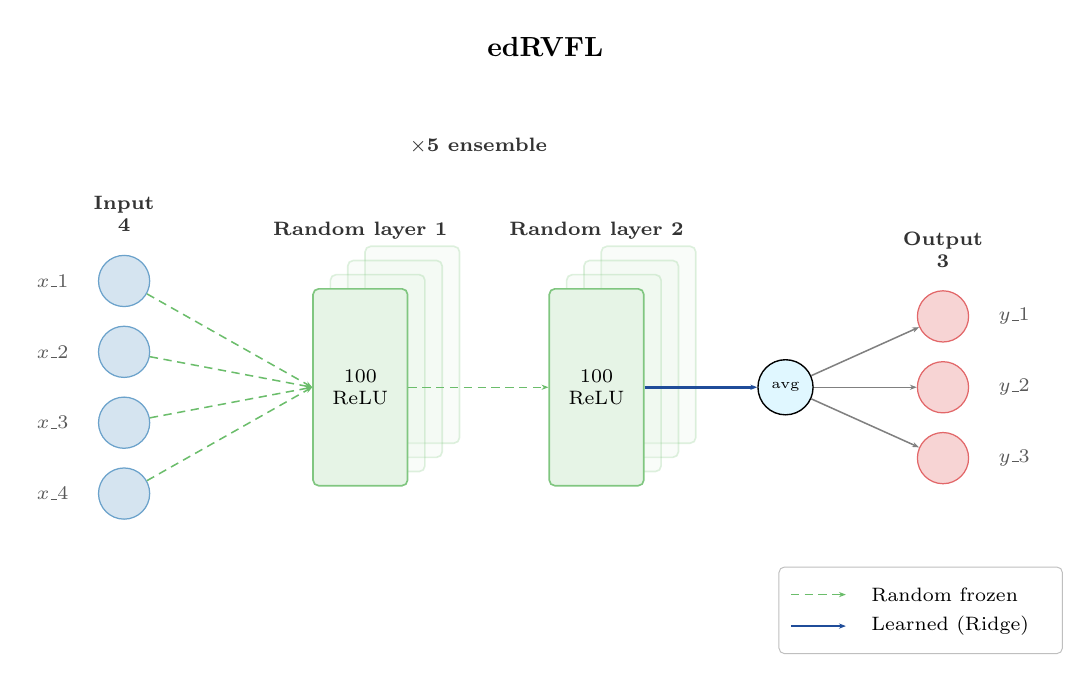
\begin{tikzpicture}
    \node[input node] (in_0) at (0.00,1.35) {};
    \node[annot, left=2.5mm of in_0] {$x\_1$};
    \node[input node] (in_1) at (0.00,0.45) {};
    \node[annot, left=2.5mm of in_1] {$x\_2$};
    \node[input node] (in_2) at (0.00,-0.45) {};
    \node[annot, left=2.5mm of in_2] {$x\_3$};
    \node[input node] (in_3) at (0.00,-1.35) {};
    \node[annot, left=2.5mm of in_3] {$x\_4$};
    \node[lbl, above=5mm] at (0.00,1.35) {Input\\4};
    \node[frozen block, opacity=0.25, fill opacity=0.25] at (3.66,0.54) {};
    \node[frozen block, opacity=0.25, fill opacity=0.25] at (6.66,0.54) {};
    \node[frozen block, opacity=0.25, fill opacity=0.25] at (3.44,0.36) {};
    \node[frozen block, opacity=0.25, fill opacity=0.25] at (6.44,0.36) {};
    \node[frozen block, opacity=0.25, fill opacity=0.25] at (3.22,0.18) {};
    \node[frozen block, opacity=0.25, fill opacity=0.25] at (6.22,0.18) {};
    \node[frozen block] (H0) at (3.00,0) {100\\ReLU};
    \node[lbl, above=5mm] at (H0.north) {Random layer 1};
    \node[frozen block] (H1) at (6.00,0) {100\\ReLU};
    \node[lbl, above=5mm] at (H1.north) {Random layer 2};
    \node[lbl, above=8mm] at (4.50,2.04) {$\times$5 ensemble};
    \node[avg node] (avg) at (8.40,0) {\tiny avg};
    \node[output node] (out_0) at (10.40,0.90) {};
    \node[annot, right=2.5mm of out_0] {$y\_1$};
    \node[output node] (out_1) at (10.40,0.00) {};
    \node[annot, right=2.5mm of out_1] {$y\_2$};
    \node[output node] (out_2) at (10.40,-0.90) {};
    \node[annot, right=2.5mm of out_2] {$y\_3$};
    \node[lbl, above=5mm] at (10.40,0.90) {Output\\3};

    \draw[random arr] (in_0) -- (H0.west);
    \draw[random arr] (in_1) -- (H0.west);
    \draw[random arr] (in_2) -- (H0.west);
    \draw[random arr] (in_3) -- (H0.west);
    \draw[random arr] (H0.east) -- (H1.west);
    \draw[learned arr] (H1.east) -- (avg);
    \draw[arr] (avg) -- (out_0);
    \draw[arr] (avg) -- (out_1);
    \draw[arr] (avg) -- (out_2);

    % legend
    \begin{scope}[shift={($(current bounding box.south east)+(0.3,-0.6)$)}]
    \fill[white, rounded corners=2pt, draw=black!25, line width=0.35pt] (0,0) rectangle (-3.6,-1.10);
    \draw[random arr] (-3.45,-0.35) -- (-2.75,-0.35);
    \node[anchor=west, font=\scriptsize] at (-2.55,-0.35) {Random frozen};
    \draw[learned arr] (-3.45,-0.75) -- (-2.75,-0.75);
    \node[anchor=west, font=\scriptsize] at (-2.55,-0.75) {Learned (Ridge)};
    \end{scope}

    % title
    \node[font=\bfseries, above=8mm] at (current bounding box.north) {edRVFL};
\end{tikzpicture}
\end{document}
